% !TEX root = migratedoc.tex
\chapter {Menu and Options}
\myabstract{Most options can be changed through the textual menu.}
You can change the options in the menu (Fig. \ref{TOPM}) using letters or in submenus numbers. 
In menu entry \texttt{ Data type} you need to specify what kind of data you have and according
to that type some other menu entries appear, for example:  transition/transversion ratio for sequences.\\

\begin{figure}[bht]

\begin{center}

\begin{boxedminipage}[t]{5.2in}
\begin{small}
%\ttfamily{
\begin{verbatim}
 ===========================================================
  POPULATION SIZE, MIGRATION, DIVERGENCE, ASSIGNMENT, HISTORY
  Bayesian inference using the structured coalescent
  ===========================================================
  Using Intel AVX (Advanced Vector Extensions)
  Compiled for a SYMMETRIC multiprocessors (GrandCentral)
  PDF output enabled [Letter-size]
  Version 4.0   [2022]
  Program started at   Tue Jul 15 11:37:15 2014


  Settings for this run:
  D       Data type currently set to: DNA sequence model            
  I       Input/Output formats and Event reporting
  P       Parameters  [start, migration model]
  S       Search strategy
  W       Write a parmfile
  Q       Quit the program


  To change the settings type the letter for the menu to change
  Start the program with typing Yes or Y
===> 
\end{verbatim}
%}
\end{small}
\end{boxedminipage}
\end{center}
\caption{\textsf{ Top menu of \textit{ Migrate}}}
\label{TOPM}
\end{figure}
Menu options can also be changed in the \texttt{ parmfile}, but before you do that, become more experienced with the
menu and its interaction with the parmfile (make some changes in the menu, save the parmfile, and then check
how these changes were translated. Never ever use an old parmfile from earlier versions to edit by hand, you will miss
new options and also potential changes in the parmfile. If you want to use options of an older parmfile, load it into \migrate
and save it using the menu option, and then manipulate the parmfile with a text editor. \textbf{\migrate will overwrite currently all
user comments added to the parmfile.}
All possible options are shown in \texttt{ parmfile} syntax, but the same items can 
be changed in the menu as well. All entries in the \texttt{ parmfile} 
are not case sensitive and all options
can be given with the first letter, e.g. datatype=Allele is equal to 
datatype=A. 
\newpage
 \section{Data type}
If you chose \texttt{ D} in the main menu then will get the data menu (Fig. \ref{DATAMENU}). More options will appear with some choices, for example when you have dated samples you can add a datefile and will also need to specify a mutation rate estimate  (Fig. \ref{DATAMENU2}). These additional options are meaningless without dated samples and should only be used with that type of ancient 
DNA or virus datasets.
\begin{figure}[bht]

\begin{center}
\begin{boxedminipage}[t]{14.5cm}
\begin{small}
\ttfamily{
\begin{verbatim}
  DATATYPE AND DATA SPECIFIC OPTIONS

  D   change Datatype, currently:                  DNA sequence model
  1   change Mutation model, currently:                Felsenstein 84
  2   Haplotyping is turned on:                                    NO
  5   One category of sites?                             One category
  6   One region of substitution rates?                           YES
  8   Sites weighted?                                              NO
 10   Sequencing error rate?                [0.000 0.000 0.000 0.000]
 11   Slow but safer Data likelihood calculation                   NO
 13   Inheritance scalar set                                       NO
 14   Pick random subset per population of individuals             NO
 15   Tip date file                     None, all tips a contemporary


  Are the settings correct?
  (Type Y or the number of the entry to change)
===> 
\end{verbatim}
}
\end{small}
\end{boxedminipage}
\end{center}
\caption{\textsf{ Data menu}}
\label{DATAMENU}
\end{figure}

\begin{figure}[bht]

\begin{center}
\begin{boxedminipage}[t]{14.5cm}
\begin{small}
\ttfamily{
\begin{verbatim}
  DATATYPE AND DATA SPECIFIC OPTIONS

  D   change Datatype, currently:                  DNA sequence model
  1   change Mutation model, currently:                    Tamura-Nei
  2   Haplotyping is turned on:                                    NO
  5   One category of sites?                             One category
  6   One region of substitution rates?     3 categories of regions
  7   Rates at adjacent sites correlated?    NO, they are independent
  8   Sites weighted?                                              NO
 10   Sequencing error rate?                [0.000 0.000 0.000 0.000]
 11   Slow but safer Data likelihood calculation                  YES
 13   Inheritance scalar set                                       NO
 14   Pick random subset per population of individuals              5
 15   Tip date file                                          datefile
 16   Mutation rate per locus and year                 0.000000100000
 17   How many generations per year                            1.0000


  Are the settings correct?
  (Type Y or the number of the entry to change)
===> 
\end{verbatim}
}
\end{small}
\end{boxedminipage}
\end{center}
\caption{\textsf{ Data menu with more options that appear with dated samples, and site rate categories}}
\label{DATAMENU2}
\end{figure}
To change the data type select \texttt{ 1}, the other numbers show
options that are relevant for the actual data type. There are several
datatypes such as the following:\\
{\bt{datatype=$<$Allele $|$ Microsatellites $|$ Brownian $|$ Sequences $|$ Nucleotide-polymorphisms $|$ 
 HapMap-SNP $|$ 
%Panel-SNP $|$ 
Genealogies $>$}}\\
specifies the datatype used for the analyses, needless to say
that if you have the wrong data for the chosen type the program
will crash and will produce sometimes very cryptic error messages.
\begin{description}
\item{\bt{Allele}:} infinite allele model, suitable for electrophoretic
markers, perhaps the ``best'' guess for 
codominant markers of which we do not know the mutation model.
\item{\bt{Microsatellite}:} a simple electrophoretic ladder model is 
used for the change along the branches in genealogy.
\item{\bt{Brownian}:} a Brownian motion approximation to 
the stepwise mutation
model for microsatellites us used (this is \textbf{ much} faster 
than exact model,
but is not a good approximation if population sizes $\Theta_i$ 
are small (say below 10).
\item{\bt{Sequences}:} Data are DNA or RNA sequences and the mutation model used is F84, first used by Felsenstein 1984 (actually the same
as in \texttt{ dnaml} \citep[Phylip version 3.5; ][]{felsenstein:1993:ppia}, a description of this model 
can be found in \cite{swofford:1996:pi}. 
\item{\bt{Nucleotide-polymorphism}:}[SNP] the data likelihood is corrected for 
sampling only variable sites. We assume that the a sequence data set
was used to find the SNP. It is more efficient to run the full sequence
data set.
\item{\bt{HapMap-SNP}:}[SNP] the data likelihood is corrected for 
sampling only variable sites. We assume that the a sequence data set
was used to find the SNP. 
%\item{\bt{Panel-SNP}:} the data likelihood is corrected for 
%using a panel of SNP sites, that were polymorphic. The panel has to be population 1. 
\item{\bt{Genealogies}:} Reads the \texttt{ bayesallfile}   (see INPUT/OUTPUT section) of a previous runs,
currently this option simply recreates the histogram, this allows the readjust some of the printouts but its usability to
create new plots is limited.
\end{description} 

\subsubsection{Sequence data}
If you specified {\bt{datatype=Sequence}} the following options have some meaning and will show up in the menu (see also details for these options in the main.html and dnaml.html of the PHYLIP distribution\\
\texttt{ http://evolution.gs.washington.edu/phylip.html})
\begin{description}
\item{\bt{ttratio=$<$ r1 r2 .....$>$}}\\ you need to specify a
transition/transversion ratio, you can give it for each locus in the
dataset, if you give fewer values than there are loci, the last
ttratio is used for the remaining loci $\rightarrow$ if you specify
just one ratio the same ttratio is used for all loci.
\item{\bt{freq-from-data=$<$ Yes $|$ No:freqA freqG freqC freqT$>$}}\\
{\bt{freq-from-data=Yes}}
 calculates the base frequencies from the infile data, this will
 crash the program if in your data a base is missing, e.g. you try
 to input only transitions. The frequencies must add up at least to 0.9999.\\
{\bt{freq-from-data=No:0.2 0.2  0.3 0.3}}
Any arbitrary nucleotide frequency can be specified.
\item{\bt{sequence-error=$<\{$VALUE,VALUE,VALUE,VALUE$\}|$Estimate:$1|4>$}\\ 
The number has to be between 0.00 and
1.00, default is 0.00, which of course is rather far from the truth of
about 0.001 (= 1 error in 1000 bases). The values are considered to be error rates for all sites and sequences. One can in principle estimate the error rate (for for all bases or 4 for each of the bases) through MCMC but this may not work well. Examples are\\
\bt{sequence-error=$\{$0.002,0.001,0.0004,0.005$\}$}\\
\bt{sequence-error=Estimate:1}}
\item{\bt{categories=$<$Yes $|$ No$>$}}\\
 If you specify {\bt{Yes}} you need a file named "\texttt{ catfile} in the same  directory
 with the following Syntax:
 number\_of\_categories cat1 cat2 cat3 .. categorylabel\_for\_each\_site
 for each locus, a \#  in the first column can be used to start a comment-line. This option is very rarely used. 
 Example is for a data set with 2 loci and 20 base pairs each
 \begin{small}
 \begin{verbatim}
 # Example catfile for two loci
 # in migrate you can use # as comments
 2 1 10         11111111112222222222
 5 0.1 2 5 23 3 11111122223333445555
\end{verbatim}
\end{small}
\item{\bt{rates=$<$ n : r1 r2 r3 ..rn$>$}}\\
by specifying rates  a hidden Markov model is used for the sequences \cite{felsenstein:1996:hmm}, also see the \textsc{ Phylip} documentation.
In the \texttt{ Menu} you can specify rates that follow
 a Gamma distribution,
with the shape parameter \texttt{ alpha} of that Gamma distribution,
the program then calculates the rates and the rate probabilities ({\bt prob-rates}). 
\item{\bt{prob-rates=$<$ n : p1 p2 p3 ... pn$>$}}\\
if you specify your own {\bt{rates}} you need also to specify 
the probability of occurrence for each rate. \migrate is using, like PHYLIP,  Laguerre quadrature points to find the discrete rates with their probability [in contrast to other programs that use discrete values at equal probabilities]

\item{\bt{autocorrelation=$<$Yes:value $|$ No$>$}}\\
if you assume hat the sites are correlated along the sequence, specify the block size, by assuming that only neighboring nucleotides are affected you would
give a value=2. [this option may not work in  version 4.x]

\item{\bt{weights=$<$Yes $|$ No$>$}}\\
If you specify {\bt{Yes}} you need a file \texttt{ weightfile} with weights for each
 site, the weights can be the following numbers 0-9 and letters A-Z,
 so you have 35 possible weights available.
 \begin{small}
 \begin{verbatim}
# Example weightfile for two loci
11111111112222222222
1111112222AAAA445XXXX5
\end{verbatim}
\end{small}
%\item{\bt{interleaved=$<$Yes $|$ No $>$}}\\
%If your data is interleaved you need to specify this here, the default is
%\bt{interleaved=No}. DO NOT USE THE INTERLEAVED FORMAT!
%\item{\bt{fast-likelihood=$<$Yes $|$ No$>$}}\\
%With very large data sets the common scheme to keep conditional
%likelihood values in the tree breaks down and a scaling factor is needed
%to get correct results. If you specify ``Yes'' the scaling factor is
%used. This comes with a penalty: the program runs about 20-40\% slower! 

%\item{\bt {usertree}=$<$NO $|$ TREE:treefile $|$ DISTANCE:distfile $|$ RANDOM $>$}\\
%The default is \textbf{NO} and \migrate calculates a starting tree using a UPGMA tree that uses a very simply distance matrix between the samples and then constrains this topology to follow a coalescent. 
%
%If you specify {\bt TREE} you need a file \texttt{ intree}. In this file you have
% starting trees for each locus. this option will accept trees with migration events in it
% but they are not needed and \migrate will insert a minimal number of them. [This needs still more testing].
%
%You can supply a \textbf{DISTANCE} file for each locus (using PHYLIP syntax).
%Each individual must have is own name; this only works with sequences. 
%The distance file is then used to create an UPGMA tree with a minimal number of migration events. For large trees this is options help to get 
%better starting trees than the automatic tree generation which uses
%a rather unsophisticated distance method (differences).
%
%With the keyword \textbf{RANDOM} one can generates a random starting tree with ``coalescent time intervals''  according to the start parameters. This is generally a bad choice,  but in conjunction of many short chains and the \textbf{ replicate=YES:number} 
%option [number is bigger than 1, see below]. This can help to search the 
%parameter space more efficiently.

\item \textbf{ inheritance-scalars=\{value1, value2, ....\}} 
The inheritance scalar is relative to the locus that is set to 1.0. If that locus is a nuclear marker and the species is diploid then all $\Theta$ are equivalent to $4N_e\mu$, if that locus is a segment of mtDNA then all $\Theta$ are equivalent to $N_e\mu$ (maternal inheritance, sex ratio 1:1). If you have 3 loci, for example in this order: a nuclear marker, a mtDNA marker, and an X-linked marker then the input for this option is:\\
inheritance-scalars=\{1.0, 0.25, 0.75 \}\\
This expresses all loci as $\Theta=4N_e\mu$; A second example: if you have two loci, the first is Y-chromosome segment and the second is X-linked and you would want to express all in $\Theta_Y$ then \\
inheritance-scalars=\{1.0, 3.0 \}\\
or if you want to express in $\Theta_X$ then\\
inheritance-scalars=\{0.333 1.0\}\\
Use for the reference locus the scalar 1.0 and all other scalars relative to that.

\item \textbf{ random-subset=$<$NO $|$ number$>$}
\migrate can randomly subsample each population. Picking the number specified in the \textbf{ random-subset}. If the population sample has fewer individuals than the specified number, all samples are taken for that population.


\item\textbf{ tipdate-file}= $<$NO $|$ YES:datefile $>$ \\
IF YOU HAVE ONLY CONTEMPORARY DATA DO NOT USE THIS OPTION.\\
The \texttt{ datefile} contains sampling-dates for the individuals (the tips of the genealogy). An example is this: 
\texttt{ tipdate-file=YES:datefile.bison3}\\
The datefile format is close to the \texttt{ infile} format but for obvious content reasons not identical, in generalized form it looks like this:
 \begin{small}
 \begin{verbatim}
 <Number of populations> <Number of loci>  <Title>
<Number of individuals>  <Population title>
<individual1 1-10>      <Date>  
<individual2 1-10>      <Date>  
<individual3 1-10>      <Date>  
....
<Number of individuals>  <Population title>
<individual4 1-10>      <Dual Date>  
<individual5 1-10>      <Dual Date>  
....
\end{verbatim}
\end{small}
The individual names MUST match the individual names in the \texttt{ infile} and all names MUST be unique, this is a stringent requirement that is only needed when you use a datefile to guarantee that the right dates and sequences are matched. 

The date must be given as a date measured backwards in time (dual time), so if a bison died 164 BC and you are able to extrac DNA from the bones then you should specify that the bison died 2172 years ago (in 2008), \migrate will adjust so that the smallest date will be set to date zero. Here an example using the mentioned syntax:
 \begin{small}
 \begin{verbatim}
 2 1  Bison priscus dated samples
3  Alaska
a2172     2172  
a2526     2526  
a4495     4495  
2 Siberia
s14605    14605
s23040    23040
\end{verbatim}
\end{small}
In the example the dates are the years before present, but in principle they can be any units as lon as the mutation rate per 'year' and the generation-per-year is on the same scale.

\item\textbf{ mutationrate-per-year}= \{$<$mutationrate1$>$,$<$mutationrate2$>$,...\}  \\
For example: mutationrate-per-year=\{0.0000005\}\\
IF YOU HAVE ONLY CONTEMPORARY DATA DO NOT USE THIS OPTION.\\
If you do not know the mutation rate, guess and try out to estimate the mutation rate in the analysis but depending on your data this may be a taxing analysis. For the moment use the mutation rate per generation and not year, see below.

\item\textbf{ generation-per-year}= $<$value$>$ \\
IF YOU HAVE ONLY CONTEMPORARY DATA DO NOT USE THIS OPTION.\\
The \texttt{ datefile} needs additional information about the spacing of the samples in time, the number of generations per year helps to get this spacing, but we also need the mutation rate (see above). 
Example: \texttt{ generation-per-year=1.000000}. Currently the generation time setting needs further tests, a generation time of 1.0 works, but other settings may fail; for the moment just use 1.0, and translate the results in years if needed.

\end{description}


\subsubsection{Microsatellite data}
Options that are used when the data are microsatellite repeat markers. \migrate uses repeat numbers internally, the infile can specify whether the data is in repeat numbers or in fragmentlength.
\migrate does not use models that behave differently with very small or very large numbers of repeats, It assumes that the mutation rate for a change from, say, 5 repeats to 6 is the same as from 245 to 246. 

\textsl{Stepwise mutation model:}
If the {\bt{datatype=Microsatellite}} is used, the following options have some meaning:\begin{description}
\item\textbf{{ include-unknown=$<$YES $|$ NO$>$}}\\ The default is {bf{NO}}. Alleles that are marked with a "?" are stripped from the analysis  with include-unknown=NO. Using YES leaves the "?" in the analysis, under some circumstances this might be the preferred way, but for most situations the unknowns can be safely stripped from the analysis.
 \item{\bt{micro-threshold=value}}\\
specifies the window in which probabilities of change are calculated
if we have allele 34 then only probabilities of a change from 34 to 35-44
and 24-34 are considered, the probability distribution is visualized in Figure \ref{MSATFIG} the higher this value is the longer you wait for your result, choosing it too small will produce wrong results. If you get 
-Infinity during runs of migrate then you need to check that
all alleles have at least 1 neighbor fewer than 10 steps apart.
If you have say alleles 8,9,11 and 35,36,39 then the default will
produce a probability to reach 11 from 35 and as a result the 
likelihood of a genealogy will be -Infinity because we multiply over
all different allele probabilities.\\
Default is {\bt {micro-threshold}=10}
\item{\bt {usertree}=$<$NO $|$  RANDOM $>$}\\
The default is \textbf{NO} and \migrate calculates a starting tree using a UPGMA tree that uses a very simply distance matrix between the samples and then constrains this topology to follow a coalescent. 

 With the keyword \textbf{RANDOM} one can generates a random starting tree with ``coalescent time intervals''  according to the start parameters. This is generally a bad choice,  but in conjunction of many short chains and the \textbf{ replicate=YES:number} 
option [number is bigger than 1, see below]. This can help to search the 
parameter space more efficiently.
\end{description}

For these following options see under \textsl{Sequence data} above.
\begin{description}
\item \textbf{ random-subset=$<$NO $|$ number$>$}
\item\textbf{ tipdate-file}= $<$NO $|$ YES:datefile $>$ 
\item\textbf{ mutationrate-per-year}= \{$<$mutationrate1$>$,$<$mutationrate2$>$,...\} 
\item\textbf{ generation-per-year}= $<$value$>$ 
\end{description}

\textsl{Brownian motion approximation:}
If the {\bt{datatype=Brownian}} is used, the following options have some meaning:\begin{description}
\item\textbf{{ include-unknown=$<$YES $|$ NO$>$}}\\ The default is {bf{NO}}. Alleles that are marked with a "?" are stripped from the analysis  with include-unknown=NO. Using YES leaves the "?" in the analysis, under some circumstances this might be the preferred way, but for most situations the unknowns can be safely stripped from the analysis.
\item{\bt {usertree}=$<$NO $|$  RANDOM $>$}\\
The default is \textbf{NO} and \migrate calculates a starting tree using a UPGMA tree that uses a very simply distance matrix between the samples and then constrains this topology to follow a coalescent. 

 With the keyword \textbf{RANDOM} one can generates a random starting tree with ``coalescent time intervals''  according to the start parameters. This is generally a bad choice,  but in conjunction of many short chains and the \textbf{ replicate=YES:number} 
option [number is bigger than 1, see below]. This can help to search the 
parameter space more efficiently.
\end{description}

For these following options see under \textsl{Sequence data} above.
\begin{description}
\item \textbf{ random-subset=$<$NO $|$ number$>$}
\item\textbf{ tipdate-file}= $<$NO $|$ YES:datefile $>$ 
\item\textbf{ mutationrate-per-year}= \{$<$mutationrate1$>$,$<$mutationrate2$>$,...\} 
\item\textbf{ generation-per-year}= $<$value$>$ 
\end{description}

\subsubsection{Allozyme data}
\begin{description}
\item\textbf{{ include-unknown=$<$YES $|$ NO$>$}}\\ The default is {bf{NO}}. Alleles that are marked with a "?" are stripped from the analysis  with include-unknown=NO. Using YES leaves the "?" in the analysis, under some circumstances this might be the preferred way, but for most situations the unknowns can be safely stripped from the analysis.
\item{\bt {usertree}=$<$NO $|$  RANDOM $>$}\\
The default is \textbf{NO} and \migrate calculates a starting tree using a UPGMA tree that uses a very simply distance matrix between the samples and then constrains this topology to follow a coalescent. 

 With the keyword \textbf{RANDOM} one can generates a random starting tree with ``coalescent time intervals''  according to the start parameters. This is generally a bad choice,  but in conjunction of many short chains and the \textbf{ replicate=YES:number} 
option [number is bigger than 1, see below]. This can help to search the 
parameter space more efficiently.
\end{description}

For these following options see under \textsl{Sequence data} above.
\begin{description}
\item \textbf{ random-subset=$<$NO $|$ number$>$}
\item\textbf{ tipdate-file}= $<$NO $|$ YES:datefile $>$ 
\item\textbf{ mutationrate-per-year}= \{$<$mutationrate1$>$,$<$mutationrate2$>$,...\} 
\item\textbf{ generation-per-year}= $<$value$>$ 
\end{description}


%If {\bt{datatype=Allele}} the following options have some meaning: 
%\comment{this needs checking}
%\begin{description}
%\item{\bt{delimiter=$<$Character $|$ NONE $>$}}\\
%a delimiter has to be used with microsatellite data, because the
%simple `one character'=`one allele' designation is not appropriate
%for data with huge numbers of alleles.
%If delimiter {\bt {None}} is specified the alleles are just one letter words.
%e.g. \texttt{ AA AB C?} 
%with {\bt{delimiter=.}} this would read
%\texttt{ A.A A.B C.?} but also \texttt{ 128.132 Rvs.Sahss}\\
%\comment{not working yet for electrophoretic data, but of course should too} 
%The default is {\bt{delimiter=NONE}}
%\end{description}
No special variables, but see \textbf{ Parmfile specific commands}.
\subsubsection{Nucleotide polymorphism}
Similar to \textbf{ sequence data}.
\vskip 1cm
\section{Input/Output formats}
This group of options specifies input file names and various output file options. These options are somewhat depending on the analysis methods: Maximum likelihood approach (MLA, Fig. \ref{INPUTMLA}) or Bayesian Approach (BA, Fig. \ref{INPUTBA}).
The numbering in the menus are not 1,2,3,4,... because I wanted to keep the same numbers for the options that are shared between the two approaches the same.
\begin{figure}[bht]

\begin{center}

\begin{boxedminipage}{14.5cm}
\begin{small}
\ttfamily{
\begin{verbatim}
  INPUT/OUTPUT FORMATS 
  -----------------------------------------------

  INPUT:
   1   Datafile name is                                  twoswisstowns
   2   Use automatic seed for randomisation?                       YES

  OUTPUT:
   5   Print indications of progress of run?                       YES
   6   Print the data?                                              NO
   7   Outputfile name is                                      outfile
                                                           outfile.pdf
  12   Print genealogies?                                         None
  15   Save logging information?                                    NO
  19   Show event statistics                  mighistfile (all events)
       Events are recorded every                    every sample step
       Histogram bin width                                    0.001000
  20   Record parameter change through time?               skylinefile
       Histogram bin width                                    0.001000


  Are the settings correct?
  (type Y to go back to the main menu or the letter for the entry to change)
===>\end{verbatim}
}
\end{small}
\end{boxedminipage}

\end{center}

\caption{\textsf{ Input/Output menu of \textit{ Migrate}}}
\label{INPUTBA}
\end{figure}

\subsection{Input formats}
\begin{description}
\item{\bt{infile=filename}}\\
If you insist to have a datafile names other than \texttt{ infile}, you can change
this here, if you do not specify anything here, it will use any file
with name \texttt{ infile} present in the execution directory, if there is no
\texttt{ infile} than the program will ask for the datafile and 
you can specify the path to it (this may be hard on Macs and Wintel machines). 
If you use this option, do {\bt NOT} use spaces  or ``/'' or on Macs ``:''
in your filename. The default is obviously {\bt{infile=infile}}

\item {\bt{random-seed=$<$Auto $|$ Noauto $|$  Own:seedvalue$>$}}\\
The random number seed guarantees that you can reproduce a run
exactly. I you do not specify the random number seed (\bt{seed=Auto})
the program will use the system clock. With {\bt{seed=Noauto}} the program expects to find a file named \texttt{ seedfile} with the random number seed.
With {\bt{random-seed=Own:seedvalue}} you can specify the seed value in the parmfile
(or in the menu). \\
Example for own seed:\\
\bt{random-seed=Own:21465}
If you want reproducible runs you should replace the {\bt{Auto}} seed with your own starting number (there are no requirement for the starting number perhaps except 0, ] \migrate uses the Mersenne-Twister algorithm to generate random numbers). 
The default is {\bt random-seed=Auto}. If you use
 {\bt{random-seed=Own:seedvalue}} do nor forget to change the seed for different runs,
otherwise the sequence of random numbers is always the same and the result will look the same on the same machine. 

Caution: if you run \migrate in a simulation study you should set the random number yourself, the AUTO option might produce the same random number seed for runs that are started in the same second: this is quite common under batch-queue systems, when you run the same date from the same seed, you will get always the same result. I tried to improve this by getting a better seed automatically but this is somewhat machine dependent.

\item{\bt{title=titletext}}\\
if you wish to add an informative title to your analysis,
you can do it here or in the infile, the infile will override
the title specified here. The length of the title is maximal 80 characters.
Example: {\bt{title=Migration parameter estimation of populations A and B of species X}}.
\end{description}

\subsection{Output formats}
\begin{description}
\item{\bt{progress=$<$Yes$|$No$|$Verbose$>$}} 
Show intermediate results and other hints that the program is running.
Prints time stamps and gives a prognosis when the program eventually
will finish, but this is a rather rough guide and sometimes gets fooled.
An analogy, the system knows how far to drive and how far we have 
already driven and the time, but no clue about how many speed bumps 
(many migration events) and accidents are ahead of us.
\par
Verbose adds more hints (at least for me) and information.
The default is {\bt{progress=Yes}}
\item{\bt{print-data=$<$Yes$|$No$>$}} \\
Print the data in the \texttt{ outfile}. defaults is {\bt{print-data=No}}. If you run your data for the first time trhough \migrate turn this option on, because it helps to find problems with data-reading. Especially with microsatellite data it is possible that the program runs but the loci are incorrectly read.
\item{\bt{outfile=filename}}\\
 All output is directed into this file, the default name is outfile. If you use this option, do {\bt{NOT}} use spaces  or ``/'' or on Macs ``:'' in the filename.
The default is obviously {\bt{outfile=outfile}}

\item{\bt{print-trees=$<$All $|$ None $|$ Last $|$ Best$>$ }}\\
print genealogies into \texttt{ treefile}. Remember these trees contain
migration events, \texttt{ treeview} \cite{page:1996} and \texttt{ FigTree} \cite{Rambaut:2006} can display such trees, although the migration events
do not show on these displays, other program might crash. We have a program \texttt{ eventree -- ET for short} that can display all the events on the tree, the program can be downloaded from the Migrate website.
\begin{description}

\item{{\bt{None}}:} \texttt{ treefile} is not initialized and no trees are printed, 
this is the fastest and the one I recommend.

\item{{\bt{All}}:}  will print all trees (you want to do that only for ridiculously small datasets with too short chains or you have {\bt{many Gigabytes}} of free storage).
\item{{\bt{Last}}:} Only the trees of the last long chain are printed, 
Still you will need lots of space.
\item{{\bt{Best}}:} Prints the tree with the highest data-likelihood for each locus.
This is slow! And does not give a lot of information,  except if you are more interested in the best tree for each locus than in the best parameter estimate.
\end{description}
Default is {\bt{print-trees=None}}

\item{\bt{logfile=$<$NO $|$ YES:logfilename$>$}}\\
Records the output to the screen into a file when turned on, otherwise the screen output will be lost. On windows systems this may be the only option to see what is going on the because the screen buffer is only 80 lines.

\item{\bt{mig-histogram=$<$NO $|$ $<$ALL $|$ MIGRATIONEVENTSONLY $>$:binsize:mighistfilename$>$}}\\
Records the frequencies of migration events (with MIGRATIONEVENTSONLY) or of all migration events and coalescence events (ALL) over time using \textsl{binsize}, the binsize is not optimal because you need to fix it before you know the range of times. A value 10 to 20$\times$ smaller than the average population size $\Theta$ is a good start. The output is a histogram of frequencies for each parameter, and a summary table of the average frequencies and a table of the frequency of the location of the root of the genealogy.

\item{\bt{skyline=$<$NO $|$ YES:binsize:skylinefilename$>$}}\\
\textbf{ If you have only contemporary data, do not trust this output.}
This options depends on the mig-histogram option, it uses the same binsize and needs some of its data structures, therefore do turn on the mig-histogram=ALL.... before attempt to use this option. With this option \migrate will present the changes of parameters through time, this method uses a different approach than \beast and is may be more crude but can represent migration parameters and can summarize over multiple loci.
\end{description}

\section{Start values for the Parameters}
The Parameter menu allows to change the meaning of some of the parameters and allows to set start parameters
\begin{figure}[bht]

\begin{center}

\begin{boxedminipage}{14.5cm}
\begin{small}
\ttfamily{
\begin{verbatim}
  PARAMETERS
  ---------------------------
  Start parameters:
  1   First parameter values are?
                           combined start-parameter report not finished

 Gene flow parameter and Mutation rate variation among loci:
  2   Use M for the gene flow parameter                   YES [M=m/mu]
  3   Mutation rate is                                        Constant

  Structured coalescent model and combination of localities:
  4   Sampling localities                                     default
  5   Model is set to                      Full migration matrix model
  6   Geographic distance matrix:                                   NO


  Are the settings correct?
  (Type Y to go back to the main menu or the letter for an entry to change)
===>
\end{verbatim}
}
\end{small}
\end{boxedminipage}
\end{center}
\caption{\textsf{ `Start value for the parameter' menu of \textit{ Migrate}}}
\label{STARTM}
\end{figure}

\subsection*{Start parameters}
\begin{description}
\item{\bt{theta=$<$Prior:$\{$percentvalue$\}|$ Own:$\{$value1,value2, ...$\}$ $|$ Normal:$\{$mean,std$\}|$ Uniform:$\{$minimum, maximum$\} >$}}\\
The menu option ``\textsl{Use a simple estimate of theta as start?}" allows to specify a start value for the mutation scaled population size $\Theta$. 
%With the setting {\bt{Fst}} the programs tries to use an F$_{\rm ST}$ based measure 
%%(Maynard Smith 1970, Nei and Feldman 1972)
%\citep{maynardsmith:1970:psp, nei:1972:igd}
%for the estimation of $\Theta_1$ and $\Theta_2$ which are the 4 $\times$ effective population size $\times$ mutation rate  for each population.
%The default is {\bt{theta=FST}}. The options \textbf{Normal} and \textbf{Uniform} draw start values from distributions with the specified parameters, these options can be used with the replication scheme. They inject additional variability into the start parameters, for standard runs of \migrate these options should probably not be used.
The 'prior' option is the default, it is set to 10 (=10\% of the prior value), this seems to be OK for many data sets, but this depends strongly on your prior, for example if you set an expoential prior with bounds at $0.0$ and $10^10$ then start value may be crazy high for your data. Setting prior ranges very wide is usually a bad idea.
This option is in principle not important because the MCMC run should be long enough so that the starting values do not matter. In praxis good values of start parameters allow much faster  convergence than bad ones. Simulations have shown that starting from too low values typically increases the run-length considerably, whereas to high values seem more to help than hurt, although if the start values are very large and the data is not strong then MA  can fail without a clear signal of failure; \migrate will return a large parameter estimate that does not reflect the data very well. BA is much less vulnerable to this problem. The start genealogy depends on the start parameters because even with a random topology the times are constrained to come from a coalescence process with parameters set equal to the start parameters defined here.

\item{\bt{migration=
$<$
Prior:$\{$percentvalue$\}|$Own:Migration matrix $|$ Normal:$\{$mean,std$\}|$ Uniform:$\{$minimum, maximum$\} >$}\\
The menu option \textsl{Use a simple estimate of migration rate as start?} allows to specify a start value for the migration parameter. 
%With {\bt{Fst}} the programs tries to use  an F$_{\rm ST}$ based measure 
%\citep{maynardsmith:1970:psp, nei:1972:igd, beerli:1998:emr,beerli:1999:mle}
%for the estimation of $m_1/mu$ and $m_2/mu$.
The 'prior' option is the default, it is set to 10 (=10\% of the prior value), this seems to be OK for many data sets, but this depends strongly on your prior, for example if you set an expoential prior with bounds at $0.0$ and $10^10$ then start value may be crazy high for your data. Setting prior ranges very wide is usually a bad idea.
The values for {\bt{Own}} are given in terms of $4N_em$ which is 4 $\times$ effective population size $\times$ migration rate per generation.
The default is \bt{migration=FST}. 
The \bt{migration matrix} is a $n$ by $n$ table with \textbf{ -} on the diagonal and can look 
like this for four populations
\texttt{ migration=OWN:\{ - 1.0 1.1 1.2 0.9 - 0.8 0.7 2.1 2.2 - 2.3 1.4 1.5 1.6 - \}}\\
or like this
\ttfamily{
\begin{verbatim}
migration=OWN:{ -   1.0 1.1 1.2 
               0.9 -   0.8 0.7 
               2.1 2.2 -   2.3
               1.4 1.5 1.6 - }
\end{verbatim}
}
See note on start values above under $\Theta$.}
\end{description}

\subsection*{Gene flow parameter and mutation rate variation among loci}
The gene flow parameter can be presented as $xNm$ or $M$. $M$ is the mutation scaled immigration rate $m/\mu$ that represents the importance of variability brought into the population by immigration compared with the variability created by mutation, $m$ is the fraction of the new immigrants of the population per generation. $xNm$ represents the number of immigrant per generation scaled by $x$ where $x$ depends on the data: $x=1$ for haploid, uniparental inheritance (mtDNA, Y), $x=2$ for haploids (bacteria), $x=3$ for the X chromosome in the mammal X-Y systems, $x=4$ for diploid organisms (nuclear DNA), etc. 
\begin{description}
\item \textbf{ use-M=$<$YES $|$ NO$>$}


%CONSTANT | ESTIMATE | GAMMA:alpha | OWN:loci: rate1 rate2 ... rate_loci
\item{\bt{mutation=$<$Constant $|$ Estimate$|$ Varying $|$ Relative $|$ Data $>$}}\\
If there are more than one locus the program averages the parameter distributions over all loci (this is different from the average of the most likely parameter values, loci that contribute more peaked parameter distributions are weighted more heavily than parameter distributions that have very flat distributions.]).
The mutation rate over all loci can be manipulated in a couple of ways, This options should not be used for first trials with \migrate. If you do not have DATED samples, the option 'Estimate' WILL NOT WORK. If you suspect that your data has regions of highy different mutation rates, I suggest to use the 'Relative' or 'Data' (both are the same).
The menu presents you with these choices:
\begin{small}
\begin{verbatim}
(C)onstant   All loci have the same mutation rate [default]
(E)stimate  Mutation rate 
(V)arying     Mutation rates are different among loci [user input]
(R)elative    Mutation rates estimated from data
\end{verbatim}
\end{small}
%\textsl{ONLY in Maximum likelihood Analysis}\\
% The \textbf{Gamma} flag (``estimate mutation rate") allows for the variation 
%of the mutation rate of each locus according to a Gamma distribution with
%shape parameter $\alpha$ (alpha) (which is the inverse of the square of the 
%coefficient of variation (CV) of the mutation rate, 
%CV=standard deviation / mean). 
%You need to specify a value for the shape parameter $\alpha$ (alpha). $\alpha$ values smaller than 1 suggest that most loci have few mutations but that some some can have many. If $\alpha$ is infinite the distribution is a spike, this is in principle like using the \textbf{constant} option [do not try to set alpha=infinity because \migrate will break]. For values of $\alpha > 5$ the distributions approach a normal distribution with mutation rates around a (unknown) mean.
%
%This is computationally daunting mostly for numerical reasons:
%the program is maximizing a product of integrals over all possible mutation rates for each locus likelihood.
%The Gamma option should be used carefully because when the local maximizer does not consistently find the maximum, results may be wrong.
%
%\textsl{ONLY Bayesian Analysis}\\
 The \textbf{Estimate} flag (``estimate mutation rate") allows for the variation 
of the mutation rate of each locus proposing new mutation rate values from the prior distribution.
For almost all dataset do not use this! Because you will need dated samples to estimate the mutation rate. 
%\textsl{Options for both analyses}\\
The options \textbf{ Varying} allows you to input your own mutation rate modifier. \migrate is modifying your values so that the average rate will be 1.0.

The option \textbf{ Relative} estimates a rough rate modifier for the mutation rate using the data. For sequence data the Watterson estimator is used to get relative rates, this takes into account the different numbers in the sample. For microsatellite and allozyme the allele counts are used to generate a rough value of the rate for each locus. These rates average to 1.0.

With \textbf{ Constant} no special calculations are done. The summarizing step is simply finding the 
best parameters by maximizing the sum of the log-likelihoods of each locus.
The default is {\bt{mutation=Constant}}

%Switching from BA to MA may be problematic with the gamma option not set 
\end{description}


%\subsection{${\rm F_{ST}}$ calculation (for Start value only)} 
%\textit{ Migrate} is using the ${\rm F_{ST}}$ calculation only to generate 
%starting values for the MCMC runs, when you did not wnat to give your guess-values for the parameters.
%With two population and one locus we can only calculate 3 quantities from
%the data for ${\rm F_{ST}}$: the homozygosity within each population and between them. Therefore we only can estimate 3 parameters, either both populations
%have the same size and different migration rates or the sizes can be different, but the migration rates are the same.\\
%{\bt{fst-type=$<$Theta $|$ Migration $>$}}\\
%\begin{description}
%\item{\bt{fst-type=Theta}}\\
%$\Theta$ for each population is variable, and the migration rate is fixed.
%\item{\bt{fst-type=Migration}}\\
%Migration rate for each population is variable, and $\Theta$ is fixed.
%If the number of populations in the program is bigger than 2
%only the option {\bt{fst-type=Theta}} is available. All pairwise Theta estimates are averaged. 
%\item{\bt{print-fst=$<$Yes$|$No$>$}} \\
%Print a table of an \fst estimate for comparison \cite{Beerli:1998:emr , Beerli:1999:mle} [This option is not recommended, because
%\migrate will take the liberty to insert an arbitrary value when the calculation fails, which is quite common with several populations.].
%\end{description}


\subsection{Migration model}
If you do not specify anything the posterior probability densities of all $n\times n$ parameters ($n$ mutation-scaled population sizes, and $n(n-1)$ mutation-scaled immigration rates are found) are found.
This options has many complications and is key for comparing population models. One can
\begin{itemize}
\item set particular immigration scenarios (for example, symmetric or assymetric migration, groups of migration rates with the same value)
\item force the estimation of population splitting times using a model that estimates the mean and standard deviation of population splits.
\item set some connections to zero, this allows to explore stepping stone models or other non-island-model type scenarios.
\end{itemize}

{\bt{custom-migration=$<$NONE $|$ migration-matrix$>$}}\\
The migration matrix contains the migration indicators (or divergence indicators) from population
j to i on row i, and the $\Theta$ are on the diagonal.
The migration matrix can consist of connections that are
\begin{itemize}
\item 0: not estimated
\item m: mean value of either $\Theta$ or $\M$.
\item s: symmetric migration [symmetric $\M$ not $xNm$]
\item S: symmetric migration [symmetric $\xi Nm$ not $\M$]
\item c: constant value (together with  \texttt{ migration=OWN...} 
or \texttt{ theta=OWN...})
\item * or $x$: no restriction
\end{itemize}
(the $\xi$ (xi) means a multiplier: 4 for diploid nuclear markers, 2 for haploid markers, 1 for haploid markers transmitted only through one sex, such as mtDNA and Y chromosomes)

The values can be spaced by blanks, newlines
A few examples for 4 populations:

Full model: {\bt{custom-migration=\{****\\
****\\
****\\
****\}}}\\
N-island model: {\bt{custom-migration=\{m m m    m\\
mm mm\\
m mmm\\
mmmm\}}}\\
Stepping Stone model with symmetric migrations, 
and unrestricted $\Theta$ estimates:\\ {\bt{custom-migration=\{*s00 s*s0 0s*s 00s*\}}}\\
\begin{figure}[hbt]
\begin{center}
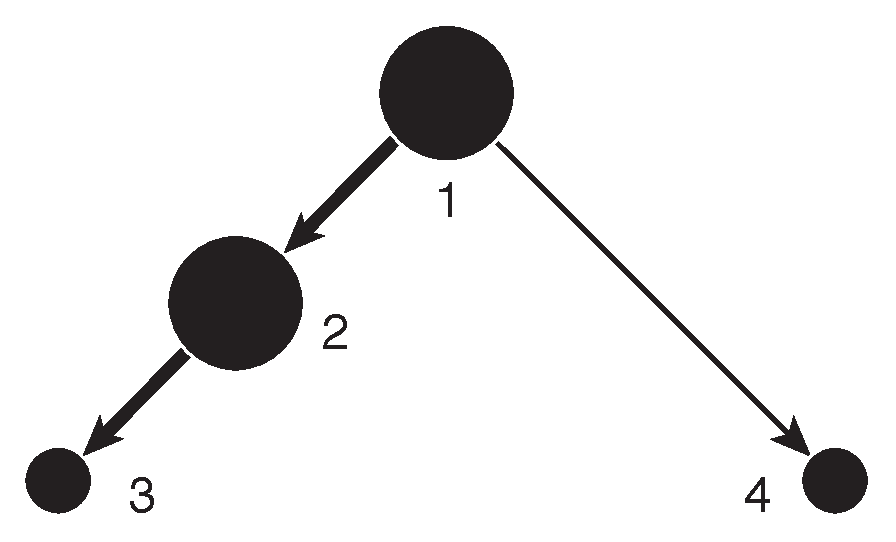
\includegraphics[scale=0.4]{mim/source_sink}
\end{center}
\caption{Source-sink example}\label{ss}
\end{figure}
Source-Sink (the first population is the source (Figure \ref{ss})):\\
{\bt{custom-migration=\{*000**000**0*00*\}}}

\subsection{Geographic distance between locations}
You can specify a distance matrix between your populations.
the distance file has the same syntax as a PHYLIP distance file [see example below].\\

{\bt{geofile=$<$NO $|$ YES:filename$>$}}\\
The distance matrix contains the distances between pairs of populations, if you choose
for example distance units in kilometers you will get migration rate estimates that are scaled
as M = immigration rate / (mutation * kilometer), if you restrict the migration rate to an average value
for all connections between population you are calculating a dispersion coefficient based on discrete
populations. This coefficient should be in the limit the same as the one calculated  from a isolation by distance population model.
\\ 
There is no requirement that the distances from i to j are the same as from j to i, although interpretation might be difficult with
an unequal distance matrix. the default filename for this distance file is \textsl{geofile}.

Example \textit{ geofile}\\
\begin{verbatim}
     3
Ermatingen0.0 10.4 12.4 
Schachen  10.4 0.0 1.0
Heiden    12.4 1.0 0.0
\end{verbatim}
\newpage
\section{Search strategy}
This section is the key to good results and you should not just use the defaults, for guidance how I myself would do this check out the section {\bt{how long to run}}.

\subsection{Maximum likelihood inference}
\begin{figure}[bh]

\begin{center}

\begin{boxedminipage}{6in}
\begin{small}
\ttfamily{
\begin{verbatim}
  SEARCH STRATEGY

  0   Strategy:                         Maximum Likelihood
  1   Number of short chains to run?                    10
  2   Short sampling increment?                         20
  3   Number of recorded genealogies in short chain?   500
  4   Number of long chains to run?                      3
  5   Long sampling increment?                          20
  6   Number of recorded genealogies in long chain?   5000
  7   Number of genealogies to discard at 
      the beginning of each chain? [Burn-in]         10000
  8   Combine chains or runs for estimates?             NO
  9   Heating:      YES (  4 chains, swap interval is   1)

 -------------------------------------------------------------
 Obscure options (consult the documentation on these)

 10   Sample at least a fraction of new genealogies?    NO
 11   Epsilon of parameter likelihood             infinity
 12   Use Gelman's convergence criterium?      YES:Summary


  Are the settings correct?
  (Type Y to go back to the main menu or the number for a menu to change)
===>
\end{verbatim}
}
\end{small}
\end{boxedminipage}
\end{center}
\caption{\textsf{ `Search strategy' menu with the Maxim likelihood approach}}
\label{SEARCHMA}
\end{figure}

\par
The terminology of {\bt{short}} or {\bt{long}} chains is arbitrary, actually
you could choose values so that short chains are longer than the ``long''
chains. Anyway, Markov chain Monte Carlo (MCMC) approaches tend 
to give better results when the start parameters are close to the maximum
likelihood values. One way to achieve this is running several short chains
and use the result of the last chain as starting value for the new chain.
This should produce better and better starting values, 
if the short chains are not too short. 

\begin{description}
\item{\bt{Strategy}}\\
With version 2.0 you have a choice of either using a maximum likelihood procedure or a Bayesian approach, on nice data both method will work about the same, for some example runs it seems that the profile likelihoods and the Bayesian posterior distribution agree quite fine on the distribution of the parameter value. The options specific to the Bayesian approach are explained in the next section.
\item{\bt{Number of short chains to run? (short-chains=value}}\\
we run most of the time about 10 short chains, which is enough if the
starting parameters are not too bad. Default is {\bt{short-chains=10}}.

\item{\bt{Short sampling increment? (short-inc=value)}}\\
The sampled genealogies are correlated to reduce the correlation between genealogies and to allow for a wider search of the genealogy space (better mixing), we sample not every genealogy, the default is {\bt{short-inc=20}}
means that we sample a genealogy and step through the next 19 and sample then
again.

\item{\bt{Number of steps along short chains? (short-steps=value)}}\\
The default number of genealogies to sample for short chains is 500.
But this may be to few genealogies for your problem. If you big data sets it
needs normally bigger samples or higher increments
to move around in the genealogy space.

\item{\bt{Number of long chains to run? (long-chains=value)}}\\
I run most of the time 3 long chains. The first equlibibrates and the last
is the one we use to estimate the parameters. Default is {\bt{long-chains=3}}.

\item{\bt{Long sampling increment? (long-inc=value)}}\\
The default is the same as for short chains. 

\item{\bt{Number of steps along long chains? (long-steps=value)}}\\
The default number of genealogies to sample for long chains is 5000.
I often choose the ``long'' chains about 10 times longer than the ``short`` chains.
\item{\bt{Number of genealogies to discard at the beginning of each chain?\\
(burn-in=value)}}\\
Each chain
inherits the last genealogy of the last run, which was created with the old parameter set. Therefore the first few genealogies are biased towards the old parameter set. When {\bt{burn-in}} is bigger than 0, the first few genealogies
in each chain are discarded. 
The default is {\bt{burn-in=10000}}.

\item\textbf{ Combine chains for estimates}
The use of this option is recommended for difficult
data sets. It allows to combine multiple chains for the parameter 
estimates when you use \textbf{ replicate=YES:LongChains}. 
With  \textbf{ replicate=YES:number} where number is, well, 
a number bigger than 1. (e.g. replicate=Yes:5), you run the program ``number'' times and the results of their last chains are combined,
The method of combination of chains is the same as in \cite{kuhner:1995:eep}
and is based on the work by \cite{geyer1991-t}. The LongChain option does not need much more time than the single chain option, but the full replication needs
exactly ``number'' times a normal run. But is sampling the search space
much better than any other option, I use this often in conjunction with
random starting trees (randomtree=YES). 
\item\textbf{ Heating (heating=$<$NO $|$ YES $|$ ADAPTIVE $<$:waitnumber:\{cold,warm,hot,boil,....\}$>$}\\
This allows for running multiple chains and swap between them, when 
these chains are run at different temperatures, 
the ``hotter'' chains explore more genealogy space than the 
``cold'' chains. An acceptance-rejection
step swaps between chains so that the the ``cold'' chains will sample
from peaks on the genealogy surface proportional to their
probability. This scheme is known as MCMCMC (Markov 
coupled Markov chain Monte Carlo),
it is based on the work of \cite{geyer:1995:amc} and uses for
four or more chains at different temperatures, the hotter chains move more freely
and so can explore other genealogies, this allows for an efficient 
exploration of data that could fit different genealogies, and should help
to set the confidence intervals more correctly than a single chain path 
could do. You need to set the temperatures yourself because there is no default.
The ADAPTIVE heating scheme manipulates these temperatures according to their
swapping success. If a neighboring temperature pair is not swapping after 1000 trials
the temperature difference between them is lowered by 10\%, if a pair is swapping more than
10 times in a 1000 the gap is increase by 10\% (these values are arbitrary, but cannot be changed in the menu, yet).
Adaptive heating is definitely no cure-it-all, I typically prefer the static heating, but it helps find good values to try for the static heating scheme, I have seen pathological behavior of long adaptive runs where all chains essentially converged to values very very close to 1.0 (the cold chain) and stopped swapping. 

If you use a STATIC heating scheme then you need to experiment a little because you want that the different
chains swap once in a while, but not too often and certainly more often
than never. The swapping seems to depend on how good the data describes a 
given genealogy. I would start with 4 chains and 
temperatures that are \textbf{ \{1. 1.5 3.0 10000.0\}}. 
The temperatures are ordered 
from cold to boiling, the coldest temperature \textbf{ MUST} be 1 (one).
The default for the heating option is \textbf{ heating=NO}. If you use
this option sampling will be at least 4 times slower, except 
if you have a multiprocessor machine and a POSIX compliant thread-library
(often called with slight variations but containing word parts such 
as pthread, thread, linuxthread), 
then you can compile the program using ``make thread'',  this will improve speed somewhat, but lately I do not gain more than 170\% CPU usage out of this. It is probably easier and faster to use all cores on new computers using the parallel version of \migrate.

The \textbf{ waitnumber} is the number of trees to wait before the differently heated chains are check whether to swap or not. I normally use 1. I have little experience whether, say, using 10 improves mixing over using 1.
\end{description}

\subsubsection{Obscure options}
If you are not experienced with MCMC or run \textit{ Migrate} for the first, 
second, ... time, do not bother about the options here.
\begin{description}
\item{\bt{Sample at least a fraction of new genealogies? ( moving-steps=$<$Yes:ratio $|$ No $>$)}}\\
With some data the acceptance ratio is very low, for example with 
sequence data with more than 5000 bp the accpetance ratio drops below 10\%
and one should increase the length of the chains. One can do this either by increasing the {\bt{long-inc}}, or {\bt{long-steps}} or by using
{\bt{moving-steps}}. The ratio means that at least that ratio of genealogies
specified in {\bt{long-steps}} have to be  new genealogies and if that fraction
is not yet reached the sampler keeps on sampling trees. In unfortunate situation this can go on for a rather long period of time.
You should always try first with the default {\bt{moving-steps=No}}.
An example:\\
You specified {\bt{long-steps=2000}},and {\bt{long-inc=20}} and the acceptance-ratio was only 0.02, you have visited 40,000 genealogies of which only 800 are new genealogies so that you have maximally sampled 800 different
genealogies for the paramter estimation.
In a new run you can try {\bt{moving-steps=Yes:0.1}}, the sampler is now extending the sampling beyond the 40000 genealogies and finally stopping when 4000 new genealogies were visited.

\item{\bt{Epsilon of parameter likelihood (long-chain-epsilon=value)}}\\
The likelihood values are ratios
\begin{align}
\frac{L(\P)}{L(\P_0)}&=\frac{1}{n} \sum_i\frac{\prob(G_i | \P)} {\prob(G_i | \P_0)}\qquad\text{(Beerli and Felsenstein, 1999)}\nonumber
\end{align}
When the Likelihood values are very similar then the ratio will be close
to 1, or 0 when we use logarithms. This means that the sampler
is not improving drastically between chains: (a) it found the maximum likelihood estimate or (b) it is so far from the maximum likelihood estimate that the surface is so flat that all likelihood values are equally bad.
using a smaller value than the default {\bt{long-chain-epsilon=100.00}}
for example a value of 1.0 would guarantee that the sampler keeps on 
sampling new long chains as long as that log-likelihood-difference drops below 1.0. In some cases this will never happen and the program will not stop.
\item{ \textbf{Gelman's convergence criterium}} If you specify ``Yes'' then 
the number of last chains get extended until the convergence criterium
of Gelman is satisfied (the ratio should be smaller than 1.2 for \textbf{ all} parameters. This can take a very long time. [In the parallel version this fails, turn it off there [this is a bug, but I had not time to find and fix it]).
\end{description}

\subsection{Bayesian method}
\begin{figure}[bht]

\begin{center}

\begin{boxedminipage}{6in}
\begin{small}
\ttfamily{
\begin{verbatim}
 SEARCH STRATEGY

   0   Strategy:                                    Bayesian Inference
   1   File for recording posterior distribution?                   NO
   2   File for recording all parameter values?                     NO
   3   Number of bins of posterior [Theta,M]?                 200, 200
   4   Plotting type of posterior distribution? up to ~100% percentile
   5   Frequency of tree updates vs. parameter updates?           0.50
   6   Proposal distribution?         Theta:Slice Mig:Slice Rate:Slice
   7   Prior distribution?            Theta:Unif. Mig:Unif. Rate:Unif.
   8   Number of long chains to run?                                 1
   9   Sampling increment?                                          20
  10   Number of recorded steps in chain                          5000
  11   Number of steps to discard at 
       the beginning of chain? [Burn-in]                         10000
  12   Running multiple replicates:                                 NO
  13   Heating:                           STATIC (  4 parallel chains)
  14   Sampling at least fraction of new genealogies:         0.000000
  15   Convergence diagnostic for replicates:              YES:Summary


  Are the settings correct?
  (Type Y to go back to the main menu or the number for a menu to change)
===>
\end{verbatim}
}
\end{small}
\end{boxedminipage}
\end{center}
\caption{\textsf{ `Search strategy' menu with the Bayesian approach}}
\label{SEARCHBA}
\end{figure}
\begin{description}
\item{\bt{File for recording parameters? (bayesfile=$<$NO $|$ YES:bayesfile$>$)}} 
this file contains the raw histogram for all parameters and all loci and their combination, figure \ref{BAYESFILE} shows the first few lines of an example, see under section \textbf{Bayesian posterior explained} further uses of this file.
\begin{figure}[bht]

\begin{center}

\begin{boxedminipage}{6in}
\begin{small}
\ttfamily{
\begin{verbatim}
# Raw data for the histogram of the posterior probabilities for all parameters
# and loci  produced by the program migrate-n 2.0.3 
# (http://evolution.gs.washington.edu/lamarc/migrate.hml)
# written by Peter Beerli 2004, Tallahassee, 
# if you have problems email to beerli@csit.fsu.edu
#
# The HPC values are indicators whether the parametervalue is in the 
# highest-posterior credibility set, a 0 means it is outside and a 1 means 
# the value is inside the credibility set.
#
# Delta for Theta and M 0.001000 0.001000 9.995000 9.995000 
# ----------------------------------------------------------------
# Locus Parameter 50%HPC  95%HPC (parameter-value count) frequency
# ----------------------------------------------------------------
1 1 0 0 0.002499 327 0.001635
1 1 0 0 0.003498 1634 0.008169
1 1 0 1 0.004498 4612 0.023058
1 1 0 1 0.005497 8970 0.044846
1 1 1 1 0.006497 13576 0.067874
1 1 1 1 0.007496 17320 0.086592
1 1 1 1 0.008496 19492 0.097451
1 1 1 1 0.009495 20537 0.102676
1 1 1 1 0.010495 19504 0.097511
\end{verbatim}
}
\end{small}
\end{boxedminipage}
\end{center}
\caption{\textsf{ First few lines of a bayesfile: the header explains the columns}}
\label{BAYESFILE}
\end{figure}

\item{\bt{File for recording all parameter values? (bayes-allfile=$<$NO $|$ YES:number:bayesallfile$>$)}}
this file contains the raw histogram for all parameters and all loci and their combination, figure \ref{BAYESALLFILE} shows the first few lines of an example, see under section \textbf{Bayesian posterior explained} for further uses of this file. This file can be very large depending on your options, it is still hard to work with files larger than 10 GB, so choose you settings carefully, there will be samples$\times$loci$\times$replicates sets of $n^2$ parameters and some additional values. If you need more samples to get good results and your data is highly autocorrelated increase the long-inc options (see there). If you specify this option (recommended) the memory foot print of the program is smaller than when this option is set to NO. This is important particularly for the parallel \migrate runs.

\begin{figure}[bht]

\begin{center}

\begin{boxedminipage}{6in}
\begin{tiny}
\ttfamily{
\begin{verbatim}
# Migrate debug 3.0 (Peter Beerli, (c) 2008)
# Raw results from Bayesian inference: these values can be used to generate
# joint posterior distribution of any parameter combination
# Writing information on parameters (Thetas, M or xNm)
# every 2 parameter-steps
# 
# --  Steps
# --  Locus
# --  Replicates
# --  log(Posterior)
# --  log(prob(D|G))
# --  log(prob(G|Model))
# --  log(prob(Model))
# --  Sum of time intervals on G
# --  Total tree length of G
# Order of the parameters:
# Parameter-number Parameter
#@      1    Theta_1
#@      2    Theta_2
#@      3    M_(2,1)
#@      4    M_(1,2)
# 
# --  Thermodynamic temperature = 1.000000
# --  Thermodynamic temperature = 1.500000
# --  Thermodynamic temperature = 3.000000
# --  Thermodynamic temperature = 1000000.000000
# --  Marginal log(likelihood) [Thermodynamic integration]
# --  Marginal log(likelihood) [Harmonic mean]
# 
#$ ------------------------------------------------------------------ 
#$ begin  [do not change this content]
#$ Model=****
#$ Mode2=****
#$ 1 2 4 0 1 1
#$ pop00
#$ pop01
#$ end
#$ ------------------------------------------------------------------ 
# 
# remove the lines above and including @@@@@, this allows to use
# Tracer (http://tree.bio.ed.ac.uk/software/tracer/) to inspect
# this file. But be aware that the current Tracer program (October 2006)
# only works with single-locus, single-replicate files
# The migrate contribution folder contains a command line utility written
# in PERL to split the file for Tracer, it's name is mba
# @@@@@@@@
#Steps  Locus   Replicate       lnPost  lnDataL lnPrbGParam     lnPrior treeintervals   treelength      Theta_1 Theta_2 M_2_1   M_1_2
100     1       1       -22365.119577   -22620.671234   255.551656      -17.034386      95      0.092424        0.00449 ...
200     1       1       -22367.961876   -22622.328216   254.366340      -17.034386      95      0.093002        0.00379 ...
300     1       1       -22368.867271   -22618.681322   249.814051      -17.034386      95      0.092687        0.00460 ...
\end{verbatim}
}
\end{tiny}
\end{boxedminipage}
\end{center}
\caption{\textsf{ First few lines of a bayesallfile: the header explains the columns, the data section is truncated at the right and bottom}}
\label{BAYESALLFILE}
\end{figure}

\item{\bt{Number of bins of posterior (\textbf{ bayes-posteriorbins=$<$thetabins Mbins $<$ratebins$>$$>$)}}}\\
The number of bins for the posterior needs to be pre-specified (to save memory). The default for $\Theta$, $M$ is 200 bins.
This number is probably to small if the range of the prior distribution is very large. If the PDF histograms look course rerun after increasing the binsizes. The ratebins are used when the mutation rate modifier with many loci is estimated in the Bayesian analysis,
this may sometimes fail, because there is little information about rate differences among loci in some datasets.

\item{\bt{Plotting bins of posterior (\textbf{ bayes-posteriormaxtype=$<$TOTAL $|$ P100$|$ P99$|$ MAXP99 $>$)}}}\\
The posterior distribution often covers only a short range of the prior distribution, therefore displaying the \textbf{ TOTAL} range of the prior distribution is often not advised, the P99 presents 99\% of the posterior distribution, cutting of 1\% of the posterior, this is a good way to visualize posterior distributions with very long (thin) right tails. P100 takes 99.99\% of the values and excludes strange outliers. MAXP99 is cutting of at 99\% credibility, but using the parameter with the highest value  for $\Theta$, and $M$, in principle this forces the same scale in the output for the parameters (this needs more testing because I most often use P100).

\item\textbf{ Frequency of tree updates versus parameter updates  (bayes-updatefreq=$<$ value $>$)}\\
The \textsl{value} specifies the ratio of genealogy updates and parameter updates, 0.5 means that the genealogy is updated roughly every second time, and one of the parameters is updated every second time. A value of 1.0 means that the parameters are never updated, A value of 0.0 is not advised because the genealogy does not adjust the migration events and so does not really test the parameter distribution for a specific tree.

\item\textbf{ Proposal distribution\\
 bayes-posterior=$<$ $<$ THETA $|$ MIG $|$ RATE $>$ $<$ SLICE $|$ METROPOLIS $>$ $>$)}\\
There are two ways the generate posterior distributions: SLICE and METROPOLIS. METROPOLIS is using the standard Metropolis-Hastings algorithm that proposes a new state not taking into account the data and then accepting or rejecting using the fit if the data to the old and new state. For some data the rejection rate is very high and many computer cycles are wasted because the MCMC chain does not move. SLICE sampling uses the current posterior distribution (taking into account the data) to generate a new state, every new state is compatible with the data, therefore the acceptance ratio is always 1.0. This comes at a price because the calculations are more demanding than the MH algorithm, and therefore may be slower. On data with lots of information SLICE sampling is great, but fails with poor data.
SLICE is the default in \migrate.
\vskip 0.5cm
Examples:\begin{small}
\begin{verbatim}
bayes-proposals= THETA SLICE Sampler
bayes-proposals= MIG SLICE Sampler
bayes-proposals= RATE SLICE Sampler
\end{verbatim}
\end{small}

\item\textbf{ Prior distribution\\
 bayes-priors=$<$ $<$ THETA $|$ MIG $|$ RATE $>$ $<$ PRIORSPECIFICATION $>$ $>$)}\\
There are several prior distribution available, but the list is still short. 
For each prior distribution you need to specify additional parameters:

\begin{tabular}{l c c c c}
Distribution & parameter 1 & parameter 2 & parameter 3 & parameter 4\\
\hline
Uniform & Minimum & Maximum & Window size & -\\
Exponential & Minimum & Mean & Maximum & -\\
Windowed Exponential & Minimum & Mean & Maximum & Window size\\
\hline
\end{tabular}
\vskip 0.5cm
Examples:\begin{small}
\vskip -0.5cm
\begin{verbatim}
bayes-priors= THETA EXPPRIOR: 0.000000 0.250000 0.500000 
bayes-priors= MIG WEXPPRIOR: 0.000000 500.000000 1000.000000 100.000000 
bayes-priors= RATE UNIFORMPRIOR: 0.010000 100.000000 5.000000 
\end{verbatim}
\end{small}
\item{\bt{Number of long chains to run? (\textbf{ long-chains=$<$value$>$)}}}\\
Use 1 long chain because multiple long chains will do little to help the analysis, if you want to combine over replicated runs use the replicate option.

\item{\bt{Sampling increment? (\textbf{ long-inc=$<$value$>$)}}}\\
Samples are taken every  \textsl{value} cycle, the default is 20. 

\item{\bt{Number of recorded genealogies in chains? (long-steps=value)}}\\
The default number of genealogies to sample for long chains is 50000. With the default increment this means
1,000,000 genealogies will be visited
This is short for many datasets.
\item{\bt{Number of genealogies to discard at the beginning of each chain?\\
(burn-in=value)}}\\
The chain is not equilibrated at the beginning of the run, and we discard those aberrant values and trees. The default is {\bt{burn-in=10000}}.

\item\textbf{ Combine chains for estimates}
The use of this option is recommended for difficult
data sets. It allows to combine multiple chains for the parameter 
estimates when you use \textbf{ replicate=YES:number}; where the number is bigger than 1. (e.g. replicate=Yes:5). 
You run the program ``number'' times and the results are combined (similar to MrBayes).
The option  \textbf{ replicate=YES:number} works for both Bayesian inference and Maximum Likelihood. The work is number times more than without replication.
For ML there is another option:  \textbf{ replicate=YES:LongChains} that allows the combination of long chains only, this is the same method as used by  \cite{kuhner:1995:eep} and is based on the work by \cite{geyer1991-t}. The LongChain option does not need much more time than the single chain option.

Replication allows a better sampling of the search space than the single chain. in particular when used on parallel cluster computers. I use this often in conjunction with random starting trees (randomtree=YES). 

\item\textbf{ Heating  (heating=$<$NO $|$ YES $|$ ADAPTIVE $<$:waitnumber:\{cold,warm,hot,boil,....\}$>$}\\
This allows for running multiple chains and swap between them, when 
these chains are run at different temperatures, 
the ``hotter'' chains explore more genealogy space than the 
``cold'' chains. An acceptance-rejection
step swaps between chains so that the the ``cold'' chains will sample
from peaks on the genealogy surface proportional to their
probability. This scheme is known as MCMCMC (Markov 
coupled Markov chain Monte Carlo),
it is based on the work of \cite{geyer:1995:amc} and uses for
four or more chains at different temperatures, the hotter chains move more freely
and so can explore other genealogies, this allows for an efficient 
exploration of data that could fit different genealogies, and should help
to set the confidence intervals more correctly than a single chain path 
could do. You need to set the temperatures yourself because there is no default.
The ADAPTIVE heating scheme manipulates these temperatures according to their
swapping success. If a neighboring temperature pair is not swapping after 1000 trials
the temperature difference between them is lowered by 10\%, if a pair is swapping more than
10 times in a 1000 the gap is increase by 10\% (these values are arbitrary, but cannot be changed in the menu, yet).
Adaptive heating is definitely no cure-it-all, I typically prefer the static heating, but it helps find good values to try for the static heating scheme, I have seen pathological behavior of long adaptive runs where all chains essentially converged to values very very close to 1.0 (the cold chain) and stopped swapping. 

If you use a STATIC heating scheme then you need to experiment a little because you want that the different
chains swap once in a while, but not too often and certainly more often
than never. The swapping seems to depend on how good the data describes a 
given genealogy. I would start with 4 chains and 
temperatures that are \textbf{ \{1. 1.5 3.0 10000.0\}}. 
The temperatures are ordered 
from cold to boiling, the coldest temperature \textbf{ MUST} be 1 (one).
The default for the heating option is \textbf{ heating=NO}. If you use
this option sampling will be at least 4 times slower, except 
if you have a multiprocessor machine and a POSIX compliant thread-library
(often called with slight variations but containing word parts such 
as pthread, thread, linuxthread), 
then you can compile the program using ``make thread'',  this will improve speed somewhat, but lately I do not gain more than 170\% CPU usage out of this. It is probably easier and faster to use all cores on new computers using the parallel version of \migrate.

The \textbf{ waitnumber} is the number of trees to wait before the differently heated chains are check whether to swap or not. I normally use 1. I have little experience whether, say, using 10 improves mixing over using 1.

\item{\textbf{Sampling at least fraction of new genealogies (moving-steps=$<$NO $|$ YES:value $>$)}}
This allows to specify that a minimum number of different genealogies need to be sampled, it is expressed as the ratio of sampled genealogies. If the frequency is not reached at the end of the specified number of samples, \migrate will continue until the ratio is satisfied, with high numbers the program may run forever. I rarely use this option.
 
\item{ \textbf{Convergence diagnostic for replicates (gelman-convergence=$<$ NO $|$ YES:$<$Sum $|$ Pairs $>$ $>$}}
This collects information about the convergence rate of two replicated chains (use two or more replicates). \textsl{Sum} reports the an average value over all whereas \textsl{Pairs} using the pairs of replicates to. Version 3.0 has some difficulties with this option and I hope to fix this in the next minor release, but on some machine and under some conditions the diagnostic fails.
 
\end{description}
%%%%%%%%%%%%%%%%%%
\subsection{Parmfile specific commands}
\subsubsection{Important parmfile options}
\begin{description}
\item{\bt{menu=$<$Yes$|$No$>$}}\\
defines if the program should show up the menu or not.
The default is {\bt{menu=Yes}}.

\item{\bt{end}}\\
Tells the parmfile reader that it is at the end of the parmfile.
\end{description}

\subsubsection{Options to change the lengths of words and texts}
If you change these, you should understand why you want to do this.
\begin{description}

\item{\bt{nmlength=number}}\\
defines the maximal length of the name of an individuum, if for a strange
reason you need longer names than 10 characters (e.g. you need more than
10 chars to characterize an individual) and you do not need this
very often then set it to a higher value, if you have no individual names
you can set this to zero (0) and no Individual names are read.
the default is {\bt{nmlength=10}}, this is the same as in PHYLIP.

\item{\bt{popnmlength=number}}\\
Is the length of the name for the population.
The default is {\bt{popnmlength=100}}

\item{\bt{allelenmlength=number}}\\
This is only used in the infinite allele case.
Length of an allele name, the default should cover even strange
lab-jargons like \texttt{ Rvf} or \texttt{ sahss} (\textit{ Rana ridibunda} very fast, \textit{ Rana saharica} super slow)
The default is {\bt{allelenmlength=6}}
\end{description}
\end{description}